\documentclass{standalone}

\usepackage{tikz,pgfplots}
\pgfplotsset{compat=newest} % change newest to current version

\begin{document}
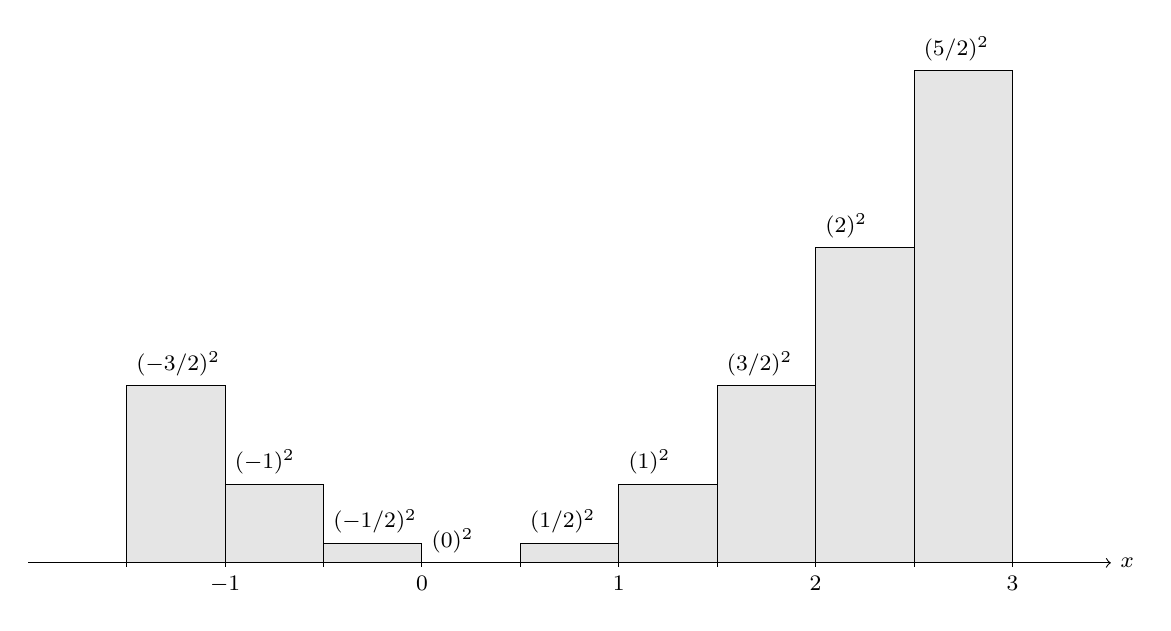
\begin{tikzpicture}[xscale=2.5]
  \draw[thin, ->] (-2,0) -- (3.5,0) node[right] {\footnotesize \(x\)};
  \foreach \x in {-1,...,3} {
    \node[below] at (\x, -0.05) {\footnotesize \(\x\)};
  }

  \foreach \x in {-3/2, -2/2, -1/2, 0, 1/2, 2/2, 3/2, 4/2, 5/2, 6/2} {
    \draw[thin] (\x, 0.05) -- (\x, -0.05);
  }

  \foreach \x in {-3/2, -2/2, -1/2, 0, 1/2, 2/2, 3/2, 4/2, 5/2} {
    \draw[fill=gray!20] (\x, 0) -- ++(0, {\x*\x}) -- ++(1/2,0) -- ++(0, -{\x*\x}) -- ++(-1/2,0);
  }
  \node[above right] at ({-3/2}, {3/2*3/2}) {\footnotesize \((-3/2)^{2}\)};
  \node[above right] at ({-2/2}, {2/2*2/2}) {\footnotesize \((-1)^{2}\)};
  \node[above right] at ({-1/2}, {1/2*1/2}) {\footnotesize \((-1/2)^{2}\)};
  \node[above right] at ({-0/2}, {0/2*0/2}) {\footnotesize \((0)^{2}\)};
  \node[above right] at ({+1/2}, {1/2*1/2}) {\footnotesize \((1/2)^{2}\)};
  \node[above right] at ({+2/2}, {2/2*2/2}) {\footnotesize \((1)^{2}\)};
  \node[above right] at ({+3/2}, {3/2*3/2}) {\footnotesize \((3/2)^{2}\)};
  \node[above right] at ({+4/2}, {4/2*4/2}) {\footnotesize \((2)^{2}\)};
  \node[above right] at ({+5/2}, {5/2*5/2}) {\footnotesize \((5/2)^{2}\)};
\end{tikzpicture}
\end{document}
